\documentclass[10pt,a4paper]{article}\usepackage[]{graphicx}\usepackage[]{color}
%% maxwidth is the original width if it is less than linewidth
%% otherwise use linewidth (to make sure the graphics do not exceed the margin)
\makeatletter
\def\maxwidth{ %
  \ifdim\Gin@nat@width>\linewidth
    \linewidth
  \else
    \Gin@nat@width
  \fi
}
\makeatother

\definecolor{fgcolor}{rgb}{0.345, 0.345, 0.345}
\newcommand{\hlnum}[1]{\textcolor[rgb]{0.686,0.059,0.569}{#1}}%
\newcommand{\hlstr}[1]{\textcolor[rgb]{0.192,0.494,0.8}{#1}}%
\newcommand{\hlcom}[1]{\textcolor[rgb]{0.678,0.584,0.686}{\textit{#1}}}%
\newcommand{\hlopt}[1]{\textcolor[rgb]{0,0,0}{#1}}%
\newcommand{\hlstd}[1]{\textcolor[rgb]{0.345,0.345,0.345}{#1}}%
\newcommand{\hlkwa}[1]{\textcolor[rgb]{0.161,0.373,0.58}{\textbf{#1}}}%
\newcommand{\hlkwb}[1]{\textcolor[rgb]{0.69,0.353,0.396}{#1}}%
\newcommand{\hlkwc}[1]{\textcolor[rgb]{0.333,0.667,0.333}{#1}}%
\newcommand{\hlkwd}[1]{\textcolor[rgb]{0.737,0.353,0.396}{\textbf{#1}}}%

\usepackage{framed}
\makeatletter
\newenvironment{kframe}{%
 \def\at@end@of@kframe{}%
 \ifinner\ifhmode%
  \def\at@end@of@kframe{\end{minipage}}%
  \begin{minipage}{\columnwidth}%
 \fi\fi%
 \def\FrameCommand##1{\hskip\@totalleftmargin \hskip-\fboxsep
 \colorbox{shadecolor}{##1}\hskip-\fboxsep
     % There is no \\@totalrightmargin, so:
     \hskip-\linewidth \hskip-\@totalleftmargin \hskip\columnwidth}%
 \MakeFramed {\advance\hsize-\width
   \@totalleftmargin\z@ \linewidth\hsize
   \@setminipage}}%
 {\par\unskip\endMakeFramed%
 \at@end@of@kframe}
\makeatother

\definecolor{shadecolor}{rgb}{.97, .97, .97}
\definecolor{messagecolor}{rgb}{0, 0, 0}
\definecolor{warningcolor}{rgb}{1, 0, 1}
\definecolor{errorcolor}{rgb}{1, 0, 0}
\newenvironment{knitrout}{}{} % an empty environment to be redefined in TeX

\usepackage{alltt}
\usepackage[latin1]{inputenc}
\usepackage{amsmath}
\usepackage{amsfonts}
\usepackage{amssymb}
\author{Erika Martínez}
\title{Guías prácticas}
\IfFileExists{upquote.sty}{\usepackage{upquote}}{}
\begin{document}

\maketitle
\newpage

UNIDAD 4: Practica 17 - Inferencia estad?stica, Estimaci?n.

SIMULACION DEL CONCEPTO DE INTERVALO DE CONFIANZA PARA ESTIMAR UN PARAMETRO.
Ejemplo 1. 
\begin{knitrout}
\definecolor{shadecolor}{rgb}{0.969, 0.969, 0.969}\color{fgcolor}\begin{kframe}
\begin{alltt}
\hlcom{#Sea la variable aleatoria X = el n?mero de caras obtenidas, al lanzar una moneda }
\hlcom{#balanceada 20 veces. Simulamos 50 muestras para generar intervalos de 95% de }
\hlcom{#confianza y as? poder estimar la proporci?n verdadera de caras (p), y encontrar }
\hlcom{#en cu?ntos de estos intervalos se encuentra el verdadero valor de la proporci?n}

\hlstd{simulIntProp} \hlkwb{<-} \hlkwa{function}\hlstd{(}\hlkwc{m}\hlstd{=}\hlnum{5}\hlstd{,} \hlkwc{n}\hlstd{=}\hlnum{1}\hlstd{,} \hlkwc{p}\hlstd{,} \hlkwc{nivel.conf}\hlstd{=}\hlnum{0.95}\hlstd{)}
\hlstd{\{}
  \hlstd{X} \hlkwb{<-} \hlkwd{rbinom}\hlstd{(m, n, p)}
  \hlcom{# Matriz con 1000 valores aleatorios binomial(n,p), 50 muestras cada una de tama?o 20 }
  \hlstd{pe} \hlkwb{<<-} \hlstd{X}\hlopt{/}\hlstd{n}
  \hlcom{# Calcula la proporci?n estimada en cada una de las muestras. }
  \hlstd{SE} \hlkwb{<<-} \hlkwd{sqrt}\hlstd{(pe}\hlopt{*}\hlstd{(}\hlnum{1}\hlopt{-}\hlstd{pe)}\hlopt{/}\hlstd{n)}
  \hlcom{# Calcula la desviaci?n est?ndarestimada en cada una de las muestras. }
  \hlstd{alfa} \hlkwb{<-} \hlnum{1}\hlopt{-}\hlstd{nivel.conf}
  \hlstd{z} \hlkwb{<<-} \hlkwd{qnorm}\hlstd{(}\hlnum{1}\hlopt{-}\hlstd{alfa}\hlopt{/}\hlnum{2}\hlstd{)}
  \hlstd{Intervalo} \hlkwb{<<-} \hlkwd{cbind}\hlstd{(pe} \hlopt{-} \hlstd{z}\hlopt{*}\hlstd{SE, pe} \hlopt{+} \hlstd{z}\hlopt{*}\hlstd{SE)}
  \hlcom{# genera los extremos del intervalo de confianza }
  \hlstd{nInter} \hlkwb{<<-} \hlnum{0}
  \hlcom{# un contador para conocer en cu?ntos intervalos se encuentra la verdadera proporci?n. }
  \hlkwa{for}\hlstd{(i} \hlkwa{in} \hlnum{1}\hlopt{:}\hlstd{m)}
    \hlkwa{if} \hlstd{((p} \hlopt{>=} \hlstd{Intervalo[i,} \hlnum{1}\hlstd{])} \hlopt{&&} \hlstd{(p} \hlopt{<=} \hlstd{Intervalo[i,} \hlnum{2}\hlstd{]))}
      \hlstd{nInter} \hlkwb{<<-} \hlstd{nInter} \hlopt{+} \hlnum{1}
  \hlcom{# funci?n que cuenta cu?ntos intervalos contienen el verdadero valor del par?metro. }
  \hlkwd{return}\hlstd{(nInter)}
\hlstd{\}}
\hlstd{n}\hlkwb{=}\hlnum{20}\hlstd{; m}\hlkwb{=} \hlnum{50}\hlstd{; p}\hlkwb{=}\hlnum{0.5}\hlstd{; nivel.conf}\hlkwb{=}\hlnum{0.95}
\hlkwd{simulIntProp}\hlstd{(m, n, p, nivel.conf)}
\end{alltt}
\begin{verbatim}
## [1] 47
\end{verbatim}
\begin{alltt}
\hlcom{#Gr?fico que muestra los intervalosde confianza de 95% que contienen y no contienen el verdadero }
\hlcom{#valor del par?metro p. }
\hlkwd{matplot}\hlstd{(}\hlkwd{rbind}\hlstd{(pe} \hlopt{-} \hlstd{z}\hlopt{*}\hlstd{SE, pe} \hlopt{+} \hlstd{z}\hlopt{*}\hlstd{SE),} \hlkwd{rbind}\hlstd{(}\hlnum{1}\hlopt{:}\hlstd{m,} \hlnum{1}\hlopt{:}\hlstd{m),} \hlkwc{type}\hlstd{=}\hlstr{"l"}\hlstd{,} \hlkwc{lty}\hlstd{=}\hlnum{1}\hlstd{)}
\hlkwd{abline}\hlstd{(}\hlkwc{v}\hlstd{=p)}
\end{alltt}
\end{kframe}
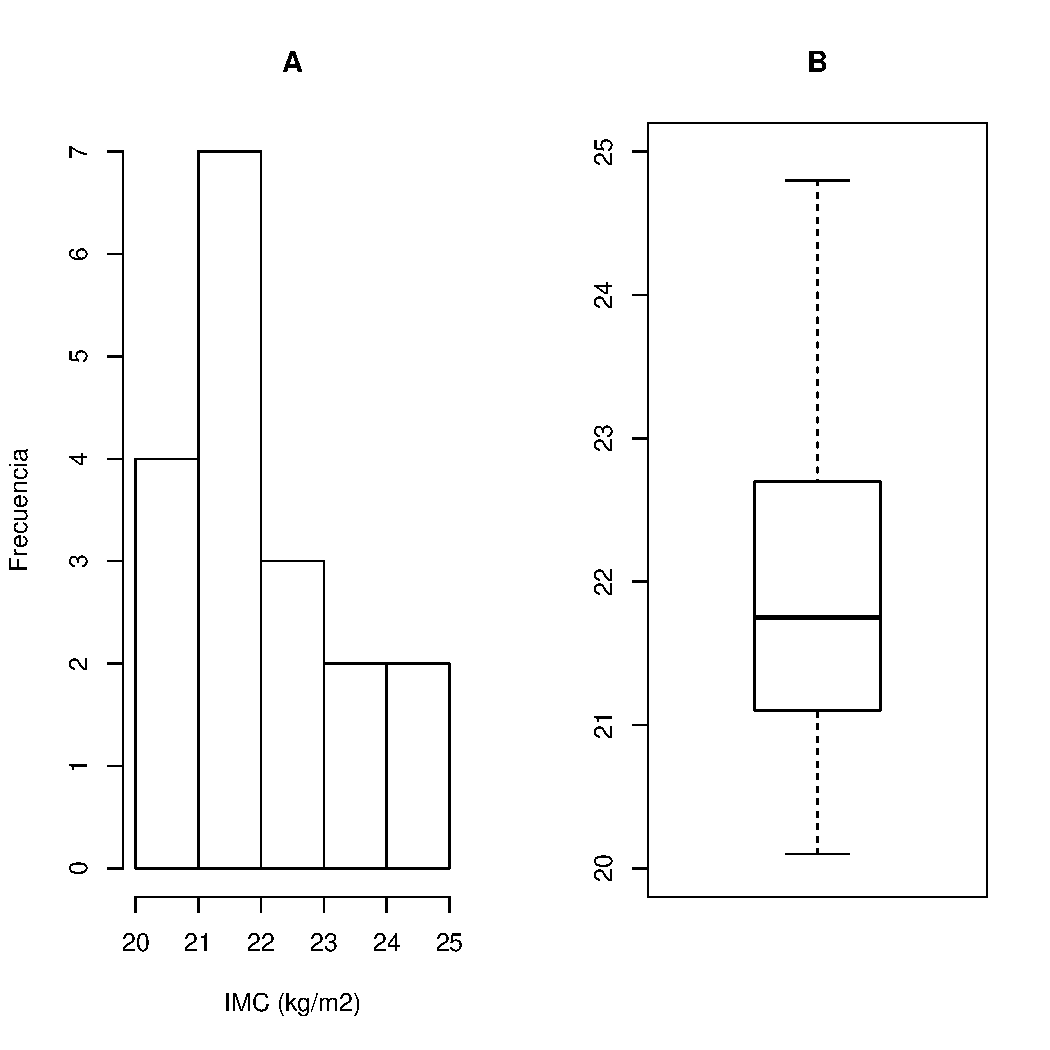
\includegraphics[width=\maxwidth]{figure/unnamed-chunk-1-1} 

\end{knitrout}

Ejercicio 1. 
\begin{knitrout}
\definecolor{shadecolor}{rgb}{0.969, 0.969, 0.969}\color{fgcolor}\begin{kframe}
\begin{alltt}
\hlcom{#Sea la variable aleatoria X = el n?mero que se obtiene al lanzar un dado no cargado }
\hlcom{#30 veces. Simular 56 muestras para generar intervalos de 95%de confianza para }
\hlcom{#estimar el promedio (??), y encontrar cu?ntos de estos intervalos contiene el valor }
\hlcom{#medio verdadero.}

\hlstd{simulIntProp} \hlkwb{<-} \hlkwa{function}\hlstd{(}\hlkwc{m}\hlstd{=}\hlnum{5}\hlstd{,} \hlkwc{n}\hlstd{=}\hlnum{1}\hlstd{,} \hlkwc{p}\hlstd{,} \hlkwc{nivel.conf}\hlstd{=}\hlnum{0.95}\hlstd{)}
\hlstd{\{}
  \hlstd{X} \hlkwb{<-} \hlkwd{rbinom}\hlstd{(m, n, p)}
  \hlcom{# Matriz con 1000 valores aleatorios binomial(n,p), 50 muestras cada una de tama?o 20 }
  \hlstd{pe} \hlkwb{<<-} \hlstd{X}\hlopt{/}\hlstd{n}
  \hlcom{# Calcula la proporci?n estimada en cada una de las muestras. }
  \hlstd{SE} \hlkwb{<<-} \hlkwd{sqrt}\hlstd{(pe}\hlopt{*}\hlstd{(}\hlnum{1}\hlopt{-}\hlstd{pe)}\hlopt{/}\hlstd{n)}
  \hlcom{# Calcula la desviaci?n est?ndarestimada en cada una de las muestras. }
  \hlstd{alfa} \hlkwb{<-} \hlnum{1}\hlopt{-}\hlstd{nivel.conf}
  \hlstd{z} \hlkwb{<<-} \hlkwd{qnorm}\hlstd{(}\hlnum{1}\hlopt{-}\hlstd{alfa}\hlopt{/}\hlnum{2}\hlstd{)}
  \hlstd{Intervalo} \hlkwb{<<-} \hlkwd{cbind}\hlstd{(pe} \hlopt{-} \hlstd{z}\hlopt{*}\hlstd{SE, pe} \hlopt{+} \hlstd{z}\hlopt{*}\hlstd{SE)}
  \hlcom{# genera los extremos del intervalo de confianza }
  \hlstd{nInter} \hlkwb{<<-} \hlnum{0}
  \hlcom{# un contador para conocer en cu?ntos intervalos se encuentra la verdadera proporci?n. }
  \hlkwa{for}\hlstd{(i} \hlkwa{in} \hlnum{1}\hlopt{:}\hlstd{m)}
    \hlkwa{if} \hlstd{((p} \hlopt{>=} \hlstd{Intervalo[i,} \hlnum{1}\hlstd{])} \hlopt{&&} \hlstd{(p} \hlopt{<=} \hlstd{Intervalo[i,} \hlnum{2}\hlstd{]))}
      \hlstd{nInter} \hlkwb{<<-} \hlstd{nInter} \hlopt{+} \hlnum{1}
  \hlcom{# funci?n que cuenta cu?ntos intervalos contienen el verdadero valor del par?metro. }
  \hlkwd{return}\hlstd{(nInter)}
\hlstd{\}}
\hlstd{n}\hlkwb{=}\hlnum{30}\hlstd{; m}\hlkwb{=} \hlnum{56}\hlstd{; p}\hlkwb{=}\hlnum{0.5}\hlstd{; nivel.conf}\hlkwb{=}\hlnum{0.95}
\hlkwd{simulIntProp}\hlstd{(m, n, p, nivel.conf)}
\end{alltt}
\begin{verbatim}
## [1] 54
\end{verbatim}
\end{kframe}
\end{knitrout}

\end{document}
